%%%%%%%%%%%%%%%%%%%%%%%%%%%%%%%%%%%%%%%%%
% Journal Article
% LaTeX Template
% Version 1.4 (15/5/16)
%
% This template has been downloaded from:
% http://www.LaTeXTemplates.com
%
% Original author:
% Frits Wenneker (http://www.howtotex.com) with extensive modifications by
% Vel (vel@LaTeXTemplates.com)
%
% License:
% CC BY-NC-SA 3.0 (http://creativecommons.org/licenses/by-nc-sa/3.0/)
%
%%%%%%%%%%%%%%%%%%%%%%%%%%%%%%%%%%%%%%%%%

%----------------------------------------------------------------------------------------
%	PACKAGES AND OTHER DOCUMENT CONFIGURATIONS
%----------------------------------------------------------------------------------------

%\documentclass[10pt]{article} % Single column

\documentclass[colorinlistoftodos,twoside,twocolumn,10pt]{article} % Two column

\usepackage{blindtext} % Package to generate dummy text throughout this template 

\usepackage[sc]{mathpazo} % Use the Palatino font
\usepackage[T1]{fontenc} % Use 8-bit encoding that has 256 glyphs
\linespread{1.05} % Line spacing - Palatino needs more space between lines
\usepackage{microtype} % Slightly tweak font spacing for aesthetics

\usepackage[spanish]{babel} % Language hyphenation and typographical rules

\usepackage[hmarginratio=1:1,top=20mm,columnsep=15mm, left=12mm, right=12mm, bottom=25mm]{geometry} % Document margins
\usepackage[hang, small,labelfont=bf,up,textfont=it,up]{caption} % Custom captions under/above floats in tables or figures
\usepackage{booktabs} % Horizontal rules in tables

\usepackage{lettrine} % The lettrine is the first enlarged letter at the beginning of the text

\usepackage{enumitem} % Customized lists
\setlist[itemize]{noitemsep} % Make itemize lists more compact

\usepackage{abstract} % Allows abstract customization
\renewcommand{\abstractnamefont}{\normalfont\bfseries} % Set the "Abstract" text to bold
\renewcommand{\abstracttextfont}{\normalfont\small\itshape} % Set the abstract itself to small italic text

\usepackage{titlesec} % Allows customization of titles
\renewcommand\thesection{\Roman{section}} % Roman numerals for the sections
\renewcommand\thesubsection{\roman{subsection}} % roman numerals for subsections
\titleformat{\section}[block]{\large\scshape\centering}{\thesection.}{1em}{} % Change the look of the section titles
\titleformat{\subsection}[block]{\large}{\thesubsection.}{1em}{} % Change the look of the section titles

\usepackage{fancyhdr} % Headers and footers
\pagestyle{fancy} % All pages have headers and footers
\fancyhead{} % Blank out the default header
\fancyfoot{} % Blank out the default footer
\fancyhead[C]{Music Genre Classifier} % Custom header text
\fancyfoot[RO,LE]{\thepage} % Custom footer text

\usepackage{titling} % Customizing the title section

\usepackage[colorlinks]{hyperref} % For hyperlinks in the PDF

\usepackage{graphicx} % For images
\usepackage{subcaption}

\usepackage{pifont} % bullets

\usepackage{amsmath}


% Keywords command
\providecommand{\keywords}[1]
{
	\small	
	\vspace{0.5em}
	\noindent \textbf{\textit{Palabras clave --- }} #1
}

%----------------------------------------------------------------------------------------
%	TITLE SECTION
%----------------------------------------------------------------------------------------

\setlength{\droptitle}{-4\baselineskip} % Move the title up

\pretitle{\begin{center}\Huge\bfseries} % Article title formatting
	\posttitle{\end{center}} % Article title closing formatting
\title{\normalsize{Proyecto Final de Aprendizaje de Máquina}\\
	\Huge\bfseries Music Genre Classifier\\
} % Article title
\author{% 
	\normalsize\textsc{Integrantes:}\\
	\normalsize\textsc{Marcos Tirador Del Riego  C-411}\\
	\normalsize\textsc{Leandro Rodr\'iquez Llosa  C-411}\\
	\normalsize\textsc{Victor Manuel Amador Sosa C-412}\\
	\normalsize\textsc{Francisco Ayra Caceres C-412}\\
	\normalsize\textsc{Ra\'ul Beltr\'an G\ómez C-412}\\
	\normalsize\textsc{Niley Gonz\'alez Ferrales  C-411}\\
	\normalsize\textsc{Arian Pazo Valido  C-311} \\[2ex]
	\small Cuarto a\~no. Ciencias de la Computaci\'on. \\ % institution
	\small Facultad de Matem\'atica y Computaci\'on, Universidad de La Habana, Cuba \\ % institution
}
\date{\footnotesize Junio 2023 } % Leave empty to omit a date


% Abstract configurations
\renewenvironment{abstract}
{\small
	\begin{center}
		\bfseries \abstractname\vspace{-.5em}\vspace{0pt}
	\end{center}
	\list{}{
		\setlength{\leftmargin}{0.9cm}%
		\setlength{\rightmargin}{\leftmargin}%
	}%
	\item\relax}
{\endlist}


\usepackage{todonotes} % \TODO
\usepackage{listings} % Code listings
\usepackage{xcolor}
\definecolor{backcolour}{rgb}{0.95,0.95,0.92}

\newcommand{\csl}[1]{\colorbox{backcolour}{\texttt{#1}}}

\newcommand{\imgcaption}[2]{\tiny \textbf{Figura #1.} #2.}

\newcommand{\mgc}[2][]{\colorbox{backcolour}{\texttt{\_\_#2\_\_#1}}}

\newcommand{\mgccapt}[1]{\texttt{\_\_#1\_\_}}

% Hyperlinks configurations
\hypersetup{
	colorlinks=true,
	linkcolor=black,
	filecolor=magenta,      
	urlcolor=cyan,
	pdftitle={Overleaf Example},
	pdfpagemode=FullScreen,
}

%----------------------------------------------------------------------------------------

\begin{document}
	% Print the title
	\maketitle

    \selectlanguage{spanish}
	\pagenumbering{gobble}
	\begin{abstract}

La clasificación de géneros musicales juega un papel crucial en las aplicaciones modernas de procesamiento de señales de audio digital. En este estudio, proponemos varios enfoques de aprendizaje automático para categorizar con precisión pistas de música en géneros predefinidos. Cada enfoque utiliza diversos conjuntos de características que se pueden extraer de las canciones; desde los comunes: MFCC, señal de audio directa; hasta características poco exploradas en este problema: letra de la canción, Transformada de Wavelet. Para evaluar los modelos utilizamos el dataset de referencia en el campo, GTZAN. En los resultados obtenidos destaca que la letra de la canción no aporta mucho a la clasificación, al menos en el dataset utilizado. Los otros modelos muestran resultados consistentes con el estado del arte, con una precisión entre $75\%$ y $80\%$

		\vspace{1em}
		\keywords{ 
			aprendizaje automático \textbf{$\cdot$} clasificación \textbf{$\cdot$}  géneros musicales \textbf{$\cdot$} MFCC  \textbf{$\cdot$} CNN  \textbf{$\cdot$} Conv1D \textbf{$\cdot$} transformada wavelet discreta \textbf{$\cdot$} transformada wavelet compleja de doble árbol  \textbf{$\cdot$} encoder  \textbf{$\cdot$} letra de canciones 
		}

	\end{abstract}
	
	%----------------------------------------------------------------------------------------
	%	ARTICLE CONTENTS
	%----------------------------------------------------------------------------------------
	
	\section{Introducción}
	La clasificación automática de géneros musicales se ha vuelto cada vez más importante debido a la gran cantidad de música digitalizada disponible en la actualidad. El etiquetado de géneros preciso permite una organización, recuperación y recomendación eficientes de canciones, allanando el camino para experiencias personalizadas en servicios multimedia. La identificación de géneros es útil para crear listas de reproducción personalizadas, analizar las preferencias de los oyentes, recomendar artistas/canciones similares, detectar material con derechos de autor e identificar estados de ánimo asociados con ciertos géneros. Sin embargo, a pesar de la gran cantidad de soluciones y avances propuestos en el procesamiento de señales musicales, persisten varios problemas para lograr sistemas de reconocimiento de género robustos y eficientes.

En primer lugar, la definición de géneros musicales sigue siendo controvertida, ya que la percepción humana varía mucho. Estas interpretaciones subjetivas conducen a anotaciones inconsistentes  y límites ambiguos entre géneros. Esta falta de consenso impide el desarrollo de modelos confiables capaces de generalizar a través de diferentes conjuntos de datos.

Aunque los géneros se derivan de influencias culturales, históricas, sociales, geográficas, tecnológicas y creativas, por lo general se reducen a etiquetas binarias. Sin embargo, muchos estilos comparten atributos y se superponen, lo que los hace difíciles de distinguir. Además, los artistas mezclan con frecuencia diferentes géneros, lo que agrega complejidad al proceso de clasificación.

En segundo lugar, la disponibilidad limitada de datos etiquetados de alta calidad plantea un gran desafío cuando se entrenan algoritmos de aprendizaje automático para la clasificación de géneros musicales. Debido al extenso tiempo que se requiere para etiquetar manualmente las pistas con géneros específicos, muchos investigadores recurren a conjuntos de datos pequeños o sintéticos, lo que lleva a modelos sobreajustados o inadecuados. Además, la obtención de colecciones más importantes a menudo implica derechos de licencia o barreras técnicas, lo que dificulta la accesibilidad y la reproducibilidad.

Por último, los enfoques actuales de aprendizaje profundo se basan en gran medida en procedimientos de preentrenamiento computacionalmente costosos, lo que los hace intensivos en recursos. Los trabajos existentes suelen utilizar servicios en la nube o potentes GPU, lo que dificulta la implementación práctica sin hardware especializado o recursos financieros. 
	  

\section {Analisis del problema}
\subsection {CNN-MFCC model}
    El problema que se pretende resolver es la clasificaci\'on de g\'eneros musicales utilizando redes neuronales convolucionales como modelo de aprendizaje y el feature MFCC como caracter\'istica extraida de los audios.
    Los MFCC se utilizan comúnmente en el procesamiento de señales de audio y voz para extraer características que se pueden utilizar en diversas aplicaciones, como el reconocimiento de voz y la clasificación de géneros musicales. Se basan en la observación de que el sistema auditivo humano es más sensible a los cambios de frecuencia en las frecuencias más bajas en comparación con las frecuencias más altas. La escala de frecuencia Mel es una transformación no lineal de la frecuencia que aproxima la respuesta del sistema auditivo humano al sonido. La razón por la que se utilizan los MFCC es que son una representación compacta del envolvente espectral de la señal de audio, lo cual es particularmente útil cuando se trata con grandes cantidades de datos de audio.
    Uno de los enfoques más populares y efectivos para abordar la clasificación de géneros musicales es utilizar los coeficientes cepstrales de frecuencia mel (MFCC) como características para representar las señales de audio.

    Los MFCC son una técnica poderosa de extracción de características para el procesamiento de señales de audio y voz y se han utilizado ampliamente en una variedad de aplicaciones, incluyendo el reconocimiento de voz, la clasificación de géneros musicales y más.
    Uno de los enfoques más populares y efectivos para abordar el problema de clasificación de géneros musicales es utilizar estos coeficientes cepstrales de frecuencia mel (MFCC) como características para representar las señales de audio.

\section {Analisis del estado del arte}
\subsection {CNN-MFCC model}
Estado del arte de MFCC, Analisis. TODO

\section {Features}
\subsection {CNN-MFCC model}
Para el entrenamiento de este modelo se utiliza el feature MFCC. Este feature es una caracter\'istica extraida de los audios popularmente utilizado para el an\'alisis de los mismos.

La razón por la que se utilizan los MFCC para entrenar el modelo es que son una representación compacta del espectro de la señal de audio, lo que es particularmente útil cuando se trabaja con grandes cantidades de datos de audio. Para calcular los MFCC, primero se segmenta la señal de audio en marcos cortos y se aplican una serie de operaciones matemáticas a cada marco, incluyendo preénfasis, enventanamiento, transformada de Fourier y compresión logarítmica, que juntas crean un conjunto de características que capturan las características más importantes de la señal de audio.

Los MFCC se pueden representar como una matriz donde cada fila corresponde a un marco particular de la señal de audio, y cada columna representa un MFCC particular.

Para la extracci\'on de MFCC en la pr\'actica se utiliza la biblioteca de python librosa, la misma posee m\'odulos espec\'ificos para la extracci\'on de la caracter\'istica MFCC de un audio.

\section{modelos}
\subsection {CNN-MFCC model}
Nuestro modelo se basa en redes neuronales convolucionales para tratar con las imágenes de MFCC. Estas redes están diseñadas específicamente para detectar patrones y características en imágenes, lo que las hace muy útiles en problemas de clasificación y reconocimiento de objetos. Las redes neuronales convolucionales son muy útiles para el procesamiento de imágenes porque son capaces de aprender patrones y características de manera automática. Esto significa que no se necesita un conocimiento experto para diseñar los filtros o características que se utilizan para procesar las imágenes, ya que la red es capaz de aprenderlos a partir de los datos de entrenamiento.

La arquitectura de una CNN se compone de varias capas de procesamiento, incluyendo capas de convolución y de pooling que permiten extraer características relevantes de las imágenes de entrada. La capa de convolución es la que aplica un filtro o kernel a la imagen de entrada para detectar patrones específicos, como bordes, líneas o texturas. La capa de pooling reduce la resolución de la imagen de salida, lo que ayuda a reducir el número de parámetros que deben entrenarse y a evitar el sobreajuste. También se usan capas independientemente de la necesidad del modelo, como capas para aplanar las imágenes a un vector, capas densas para pasarle lo que se detecto en las anteriores y ajustar pesos, y capas de activación.\\

\textbf{\large Arquitectura de capas del modelo}
\begin{itemize}
\item Capa de entrada input: recibe la la imagen con tamaño 256x192 y 3 filtros RGB.(256,192,3).

\item Capa Conv2D: recibe la capa input anterior y devuelve datos de tamaño (256,192,64), aplica 64 filtros a la imagen.

\item Capa AveragePooling2D: recibe datos de tamaño (256,192,64) y devuelve la imagen reducida en (2,2), devuelve datos de tamaño (128,96,64).

\item Capa Conv2D: recibe datos de tamaño (128,96,64) y devuelve datos de tamaño (128,96,128), aplica 128 filtros a la imagen.

\item Capa AveragePooling2D recibe datos de tamaño (128,96,128) y devuelve la imagen reducida en (2,2), devuelve datos de tamaño (64,48,128).

\item Capa Conv2D: recibe datos de tamaño (64,48,128) y devuelve datos de tamaño (64,48,256), aplicando 256 filtros a la imagen.

\item Capa GlobalAveragePooling2D: recibe datos de tamaño (128,96,128) y devuelve un vector 1D \cite{Machine Learning and Deep Learning methods for music genre Classification} de tamaño 256, con una salida por cada filtro.

\item Capa Dense de 256 neuronas: recibe los datos de la salida de la capa anterior y los procesa con la función de activación RELU.

\item Capa Dense de 128 neuronas: recibe los datos de la salida de la capa anterior y los procesa con la función de activación RELU.

\item Capa Dense de 64 neuronas: recibe los datos de la salida de la capa anterior y los procesa con la función de activación RELU.

\item Capa Dense de 32 neuronas: recibe los datos de la salida de la capa anterior y los procesa con la función de activación RELU.

\item Capa Dense de 10 neuronas: recibe los datos de la salida de la capa anterior y los procesa con la función de activación softmax para determinar la salida de tipo clasificación.
\end{itemize}

\begin{figure}
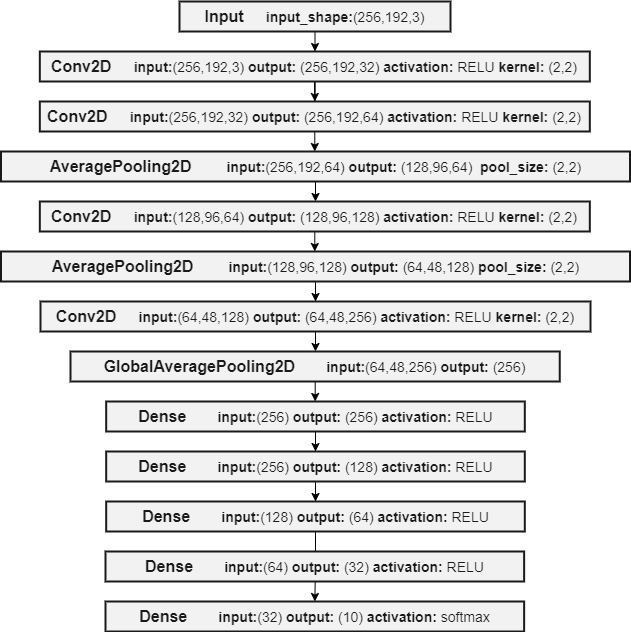
\includegraphics{CNN.png}
\end{figure}

\section{Resultados}
\subsection {CNN-MFCC model}
Tras dividir la case de datos de forma eficiente en 80\% para entrenar, 10\% para validar y 10\% para pruebas, se obtuvo como resultado de la anterior arquitectura tras 300 épocas de entrenamiento un accuracy de $0.767$ para datos de prueba, $0.819$ para datos de validación, $0.974$ para datos de entrenamiento.

Se muestran en los siguientes gráficos los resultados del entrenamiento en el transcurso de las épocas. Se puede apreciar que cuando los datos de entrenamiento "pierden" el sobreajuste, los datos de validación por lo general mejoran el resultado. En esos picos se nota cómo el modelo generaliza mejor.
  \begin{figure}
  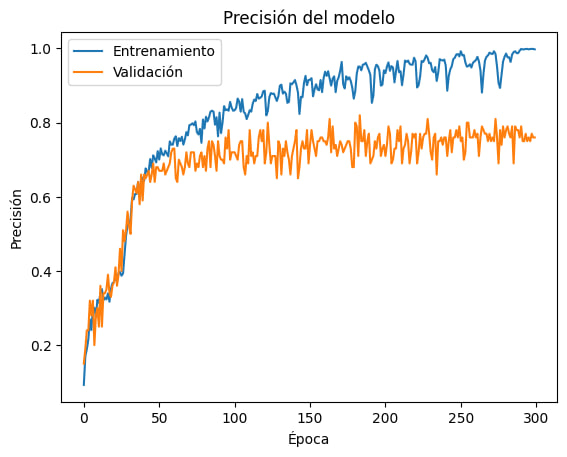
\includegraphics{CNN_accuracy.jpg}
  \end{figure}
  \begin{figure}
  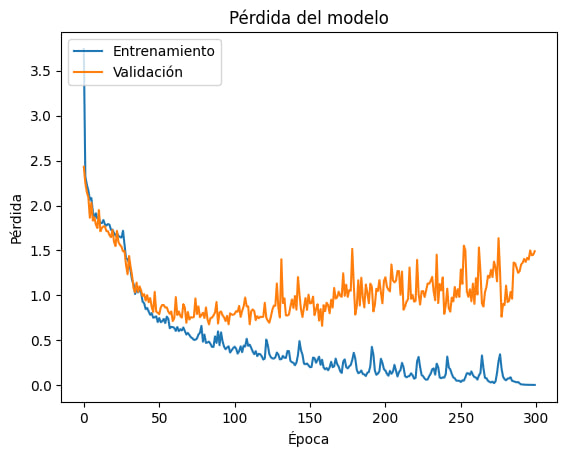
\includegraphics{CNN_loss.jpg}
  \end{figure}

  
	\section{Wavelets}

La clasificación de géneros basada en la Transformada de Fourier, utilizando MFCC y espectrogramas, se ha explorado con éxito en los últimos años. Aunque la Transformada de Fourier tiene una alta resolución en el dominio de la frecuencia, tiene una resolución cero en el dominio del tiempo. Esto significa que puede decirnos exactamente qué frecuencias están presentes en una señal, pero no en qué lugar en el tiempo se han producido \cite{wavelet transform in machine learning}. Un mejor enfoque para analizar señales con un espectro de frecuencias dinámico es la Transformada Wavelet. Esta tiene una alta resolución tanto en el dominio de la frecuencia como en el del tiempo. Además, la Transformada Wavelet puede proporcionar una resolución de frecuencia variable, lo que significa que puede adaptarse a diferentes escalas de tiempo y frecuencia. Esto puede ser útil en la clasificación de géneros musicales, donde ciertos géneros pueden tener patrones rítmicos más rápidos o lentos que otros \cite{Musical Genre Classification Of Audio Signals}. Por último, la Transformada Wavelet, ya que utiliza pocos datos para representar una señal puede ser útil en la clasificación de géneros musicales; donde el procesamiento de grandes cantidades de datos suele ser costoso en términos de tiempo y recursos computacionales. 

	Proponemos dos métodos de extracción de características usando varias formas de Transformadas Wavelet. 
    El primero es la Transformada Wavelet Discreta (DWT) \cite{wavelet transform in machine learning} y el segundo la Transformada Wavelet Compleja de Doble Árbol (DT-CWT) \cite{DT-CWT}.
    
    La DWT es un caso especial de Transformada Wavelet que proporciona una representación compacta de la señal en el tiempo y la frecuencia que se puede calcular de manera eficiente\cite{Musical Genre Classification Of Audio Signals}. La DT-CWT es una mejora relativamente reciente a DWT; ya que para señales moduladas complejas como el audio, DWT encuentra algunas pocas deficiencias: oscilaciones, varianza de desplazamiento, aliasing y falta de direccionalidad\cite{Wavelet Transform for Music Genre Classification}. 
    
    El pipeline para ambos métodos consiste en calcular las respectivas características para cada canción del dataset. Luego con la matriz obtenida se realiza un split de $80\%$ - $20\%$ y se entrena el modelo de machine learning elegido. Ajustando los hiperparámetros utilizando Cross-Validation.

	\subsection{Tests}

  Fueron probados varios modelos de machine learning tradicionales como Logistic Regression, SVC, Linear SVC, Random Forest Classifier y Gradient Boosting Classifier. Como los dos últimos se comportan mejor respecto al resto, con una precisi\'on superior en un 10\%, decidimos enfocarnos en esos modelos . 

Respecto a la Transformada Wavelet Discreta, Daubechies wavelet  empíricamente muestra el mejor comportamiento en muchas aplicaciones\cite{Wavelet Transform for Music Genre Classification}. Experimentamos con distintos órdenes de Daubechies wavelet, y db12 mostró el mejor comportamiento. Los mejores resultados para DWT fueron obtenidos con Random Forest; utilizando como parámetros: \emph{n\_estimators=100}, \emph{max\_depth=13}, \emph{bootstrap=False}. La precisión con este modelo se ubicaba alrededor de $0.77$. \\

	\begin{figure}[h!] % Start the main figure environment
			\centering
			\begin{subfigure}{0.45\linewidth} % First subfloat environment
					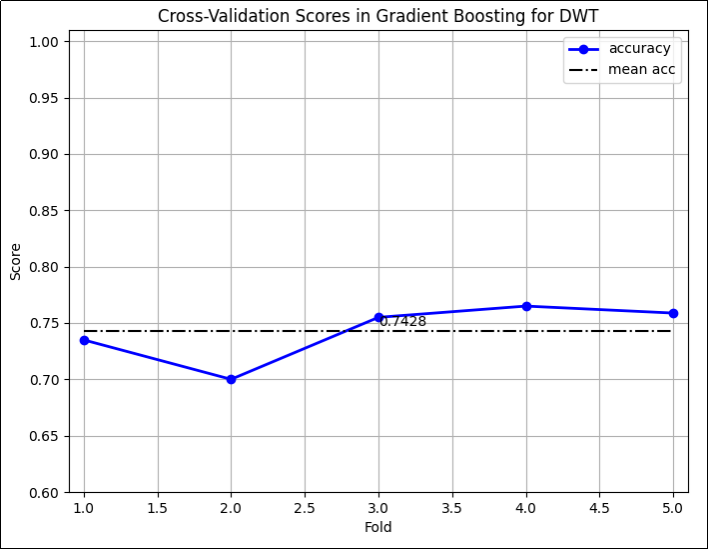
\includegraphics[width=4cm]{images/CV_DWT_gb.png}
					\caption{DWT Gradient Boosting}
				\end{subfigure}
			\hskip 1em plus 1fill minus 1fil
			\begin{subfigure}{0.45\linewidth} % Second subfloat environment
					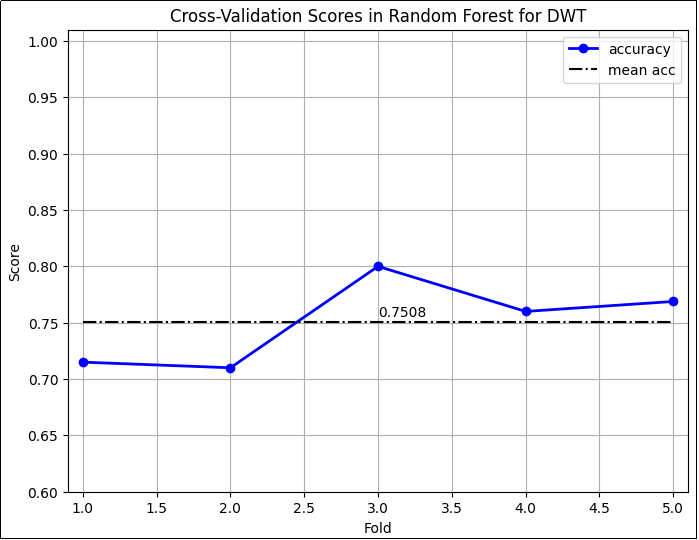
\includegraphics[width=4cm]{images/CV_DWT_rf.png}
					\caption{DWT Random Forest}
				\end{subfigure}
			\caption{DWT Cross-Validation}
		\end{figure}

La Transformada Wavelet Compleja de Doble Árbol, mostró los mejores resultados con 17 niveles de descomposición para extraer los coeficientes wavelet. Se comporta mejor que DWT, alcanzando más de $0.8$ de precisión con Random Forest Classifier.  

Además de las imagenes del Cross-Vlidation también reportamos una matriz de confusión para comprobar el comportamiento en cada género. Se observa que no se desempeña de la misma forma en todos los géneros, ya que hay algunos (como el metal o el jazz) donde se observan muy buenos resultados. \\

	\begin{figure}[h!] % Start the main figure environment
			\centering
			\begin{subfigure}{0.45\linewidth} % First subfloat environment
		
				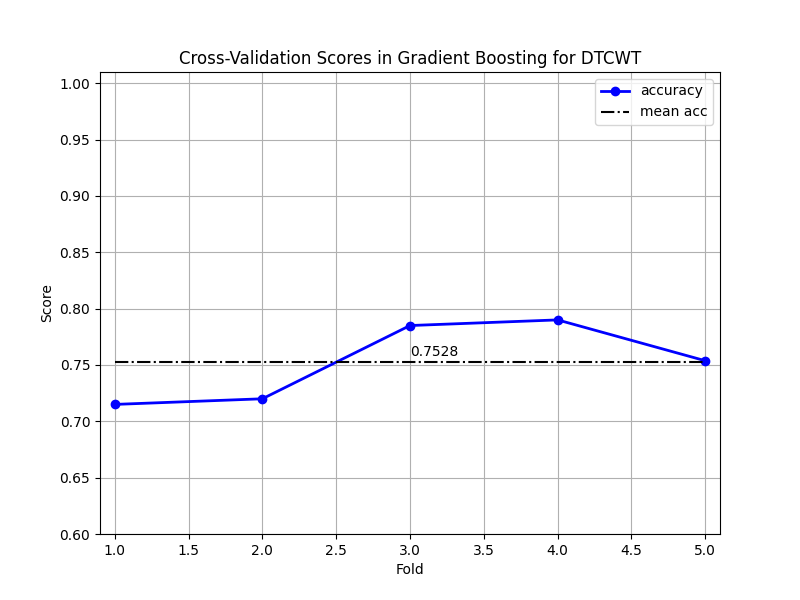
\includegraphics[width=4cm]{images/CV_DTCWT_gb.png}                   \caption{DTCWT Gradient Boosting}
				\end{subfigure}
			\hskip 1em plus 1fill minus 1fil
			\begin{subfigure}{0.45\linewidth} % Second subfloat environment
					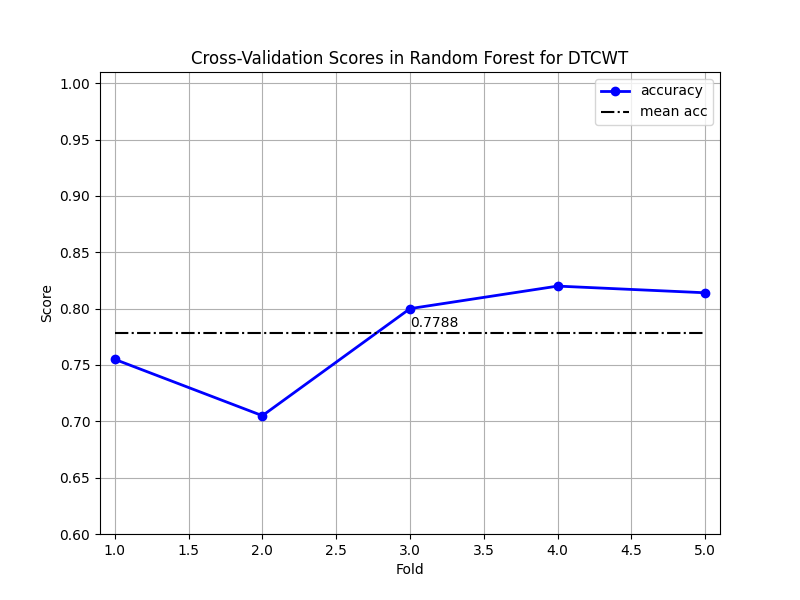
\includegraphics[width=4cm]{images/CV_DTCWT_rf.png}                   \caption{DTCWT Random Forest}
				\end{subfigure}
			\caption{DTCWT Cross-Validation}
		\end{figure}

\begin{figure}[h!] 
	\centering    
	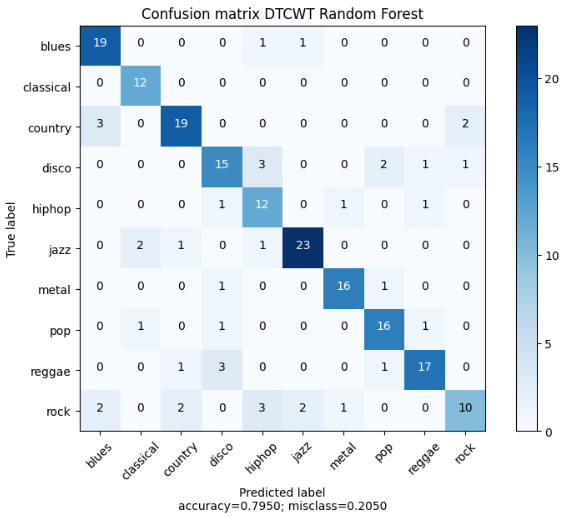
\includegraphics[width=6cm]{images/conf_matrix_DTCWT.png}    
	\caption{DTCWT Random Forest Matriz de Confusi\'on}
\end{figure}

\section{Conv1D}
Implementamos un modelo de red neuronal convolucional unidimensional (CNN 1D) para clasificar géneros de música. El modelo se basa en la arquitectura de ResNet, una popular red neuronal convolucional utilizada para tareas de clasificación. La elección de una red 1D permite al modelo procesar directamente señales de audio, lo que lo hace especialmente útil para esta tarea de clasificación de géneros musicales.

\subsection{Método}
Lo interesante y diferente en este enfoque es que, en lugar de usar características de audio pre-extraídas, el modelo aprende directamente de las formas de onda de audio. Esto puede resultar en un modelo más flexible que puede aprender representaciones más útiles para la tarea en cuestión.

La idea principal del modelo es tomar una señal de audio, pasarla a través de una serie de capas convolucionales para extraer características útiles, y luego usar esas características para clasificar la señal en uno de los géneros musicales.

El código se divide en varias partes:
\begin{itemize}
\item Carga de archivos de audio: Se usa la biblioteca librosa para cargar los archivos de audio con una frecuencia de muestreo de 22050 Hz.
\item Preprocesamiento de los datos: Los géneros se codifican en representaciones numéricas y los datos se dividen en conjuntos de entrenamiento, validación y prueba.
\item Construcción del modelo: Se define un modelo de red neuronal convolucional 1D con varias capas, incluyendo capas convolucionales, una capa de agrupación (pooling), y una capa densa (fully connected).
\item Entrenamiento del modelo: El modelo se entrena en los datos de entrenamiento, utilizando una función de pérdida de entropía cruzada categórica y el optimizador Adam.
\end{itemize}

\subsection{Comentarios}
Sin embargo, cabe mencionar que, aunque el modelo está inspirado en la arquitectura ResNet, la implementación en el código no incluye las conexiones de atajo (shortcut connections) que caracterizan a ResNet. Estas conexiones permiten que las señales pasen directamente a través de la red, ayudando a combatir el problema del desvanecimiento del gradiente durante el entrenamiento de redes profundas. A pesar de la ausencia de estas conexiones, el modelo aún puede ser efectivo para la tarea de clasificación de géneros de música. Los trabajos futuros podrían considerar la implementación de las conexiones de atajo para recrear más fielmente la arquitectura ResNet y potencialmente mejorar el rendimiento.

\subsection*{Integración en Google Colab}

El ensamblaje del modelo de entrenamiento que implementamos de Red Neuronal Convolucional 1D, o Conv1D, fue realizado en Google Colab. Este proceso fue necesario debido a la falta de recursos para el entrenamiento de la estructura de datos necesaria. También nos beneficiamos de la capacidad de Google Colab para manejar las multiplicaciones de inmensas matrices que se realizan durante los algoritmos de propagación hacia adelante y hacia atrás en el entrenamiento de la red.

El modelo es entregado en formato Jupyter Notebook (extensión .ipynb), lo que facilita la claridad y separación en módulos, así como la ejecución de partes específicas del código según sea necesario. Para una ejecución más fácil del modelo, se recomienda ejecutar el notebook desde Google Colab. Esto agilizará las descargas necesarias y evitará la necesidad de instalar módulos como 'tensorflow' y 'numpy', que ya están incluidos en el entorno de ejecución de Python en Google Colab.

La ejecución y el entrenamiento del modelo se dividen en cuatro partes fundamentales:

\begin{enumerate}
\item Importación de la biblioteca 'os' de Python.
\item Sincronización con Google Drive.
\item Descarga e importación del dataset GTZAN.
\item Entrenamiento del modelo.
\end{enumerate}

\subsection*{1. Importación de la biblioteca 'os' de Python}

La importación de la biblioteca 'os' de Python es necesaria para trabajar con el dataset de forma local después de la descarga.

\subsection*{2. Sincronización con Google Drive}

La sincronización con la cuenta de Google Drive nos permite trabajar con el dataset desde la nube, evitando la necesidad de descargarlo a nuestra PC. Una vez que se ejecuta el código identificado en el notebook para este propósito, nuestro almacenamiento en Google Drive será accesible.

\subsection*{3. Descarga e importación del dataset GTZAN}

El código para descargar e importar el dataset GTZAN solo necesita ser ejecutado una vez. Después de descargar el dataset GTZAN, lo tendremos localmente para usarlo cuantas veces sea necesario.

La descarga se realiza desde Kaggle, una plataforma que proporciona una gran cantidad de datasets y ofrece una API que nos permite descargar casi todos ellos. Los pasos detallados para descargar el dataset GTZAN desde Kaggle se explican en el notebook.

\subsection*{4. Entrenamiento del modelo}

Inicialmente, concebimos el entrenamiento del modelo trabajando directamente con los audios. Sin embargo, al investigar la clasificación de géneros musicales y trabajar con música en general, optamos por trabajar con histogramas de las canciones. Aunque dejamos ambos enfoques en el modelo, es importante solo ejecutar uno de los dos. Las instrucciones detalladas para el entrenamiento del modelo se encuentran en el notebook.

\section{Modelo VisionLang}

Hasta ahora hemos implementado algunas de las ideas m\'as exitosas para clasificar g\'eneros musicales que se pueden encontrar en el estado del arte. Pero resulta que ninguna de estas hace uso de la letra de la canci\'on, la cu\'al sabemos intuitivamente que puede aportar bastante informaci\'on sobre el g\'enero de la canci\'on. Por tanto, una idea implementada en este trabajo es hacer un modelo clasificador que conste de una red neuronal que combina análisis de la letra, mediante un embedding que represente a la misma, y de la música con un encoder. La idea de este modelo es concatenar los vectores resultantes de estos procesamientos y clasificar en base a esta combinación de features. Al mismo lo llamamos como VisionLang.

\subsection{Autoencoder}
Para construir el encoder se programó un autoencoder y se tomó el modelo hasta el bottleneck para sacar el encoder. La arquitectura del autoencoder combinó capas maxpooling y upsampling al inicio y al final respectivamente para moderar el tamaño la imagen, intercaladas con capas convolucionales y en el medio tuvo un par de capas densas para aprovechar que ya el número de dimensiones era relativamente pequeño y realizar un poco más de aprendizaje. Se tomó como función de pérdida y métrica el error cuadrático medio ($\textit{mean squared error}$). La entrada del autoencoder y la salida esperada fueron las imágenes del feature MFCC del conjunto de entrenamiento luego de haber sido normalizadas, es decir, que en vez de estar en el rango $[0, 255]$ cada valor de la imagen de entrada, los representamos en el rango $[0, 1]$. 

Anteriormente se probaron otras arquitecturas, desde algunas que no tenían capas densas hasta otras que principalmente consistían en capas densas. El problema en las arquitecturas carentes de capas densas era que sus resultados no eran lo suficientemente buenos, es decir, debido a su relativamente baja cantidad de parámetros el nivel de aprendizaje que podían lograr era inferior al que se logró luego con arquitecturas con capas densas. Por otro lado, las arquitecturas que consistían principalmente en capas densas tenían problemas como que los modelos eran muy grandes, algunos pasando de los GiB de almacenamiento y presentaban un problema para nosotros a la hora del entrenamiento. Otro problema que tienen las arquitecturas más basadas en capas densas es su tendencia al overfitting. En las prueba realizadas, las arquitecturas carentes de capas densas no presentaban este tipo de problema ya que los resultados en los conjuntos de entrenamiento, test y validación tenían poca diferencia entre ellos, sin embargo en las arquitecturas que tenían capas densas, por el gran número de parámetros si se evidencia una diferencia sustancial entre los resultados en los conjuntos de entrenamiento, y los obtenidos en los de prueba y validación. Al entrenar se realizó un $save$ cada $10$ epochs. Veamos los resultados sobre el número del $save$ en el modelo de autoencoder presentado:

\begin{figure}[h!]
	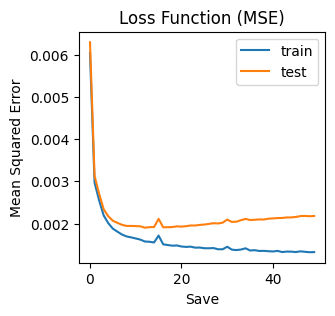
\includegraphics[width=5cm]{overfitting_graph.png}
\end{figure}

A partir del análisis de la gráfica anterior se tomó como cantidad de epochs a ejecutar la cantidad de $150$, ya que se conjeturó (y luego validó) que el comportamiento del modelo en el conjunto de prueba sería muy similar al comportamiento en el conjunto de validación y en este punto es que se obtiene un mejor performance en el conjunto de prueba. 

Volviendo atrás, los resultados obtenidos para cada tipo de modelo:
\begin{itemize}
	\item los modelos que no tenían capas densas lograron primeramente un error (MSE) de $0.0025$ y luego de ampliar la   cantidad de dimensiones que salen del bottleneck, es decir la cantidad de dimensiones de la representación se logró $0.0021$. Estos modelos tenían muy poco overfitting luego de $500$ epochs.
	\item los modelos que presentan capas densas, por su parte, comenzaron con resultados en el conjunto de entrenamiento de hasta $0.0011$ con $500$ epochs, lo cual era muy bueno pero podía implicar overfitting. A medida que se redujeron la cantidad de parámetros (de $288$ millones a los $2.3$ millones del modelo propuesto) los resultados en el conjunto de entrenamiento fueron peores pero nunca sobrepasaron el valor de $0.0013$ en $500$ epochs. Luego de correr el modelo propuesto solo $150$ epochs se obtuvieron los mejores resultados tanto en el conjunto de prueba como en el validación, oscilando alrededor de $0.00185$, por su lado en el conjunto de entrenamiento se obtuvieron resultados alrededor de $0.0016$, lo que evidencia la presencia de overfitting.
\end{itemize}

Se realizó también cross validation con Kfold dividiendo todo el conjunto de entrenamiento en $10$ subconjuntos. Los resultados del cross validation coincidieron con los resultados anteriormente descritos. Este test se hizo luego de haber fijado la cantidad de epochs en $150$.

\subsection{Feature: Letra de la canci\'on}

La segunda mitad de la informaci\'on de la que queremos que nuestro modelo aprenda es la letra de la canci\'on. Para ello lo primero que se hace es extraer la misma haciendo uso del conocido modelo de Whisper (ver \cite{whisper}). Luego necesitamos un embedding que represente al texto de la canci\'on que servir\'a de entrada al modelo. Para extraer el mismo hacemos uso de otro modelo de aprendizaje de m\'aquinas conocido como Bert (ver \cite{bert}). Este \'ultimo es un modelo basado en redes neuronales para el procesamiento de lenguaje natural, desarrollado por Google.

\subsection{Arquitectura del modelo}

Una vez obtenidos los dos embedding correspondientes a la letra de la canci\'on y la m\'usica (MFCC) ya tenemos la capa de entrada de nuestra red neuronal. La misma es la concatenaci\'on de los dos vectores obtenidos. Luego la red tiene  dos capas ocultas con funci\'on de activaci\'on RELU y cantidad de neuronas $128$ y $64$ respectivamente. Finalmente la capa de salida consiste de $10$ neuronas que representan a cada uno de los g\'eneros musicales que analizamos, y cuenta con softmax como funci\'on de activaci\'on. Siendo coherente con esto \'ultimo usamos como funci\'on de p\'erdida la Categorical Cross Entropy. Adem\'as, el modelo fue entrenado durante $500$ epochs.


\subsection{Resultados}

Como podemos ver en la siguiente gr\'afica el valor de accuracy de nuestro modelo para el training set es casi perfecto llegados al epoch n\'umero $300$. En el caso del conjunto de  datos de validaci\'on, que es el que nos da la efectividad de nuestro modelo, vemos que el accuracy crece r\'apidamente hasta llegar al valor $0.57$ alrededor del epoch $150$.

\begin{figure}[h!]
	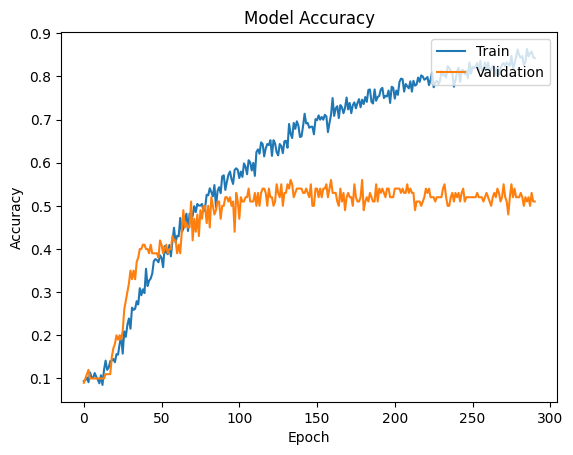
\includegraphics[width=5cm]{vl_accuracy.png}
\end{figure}

Con m\'as capas y neuronas en nuestro modelo, este hac\'ia r\'apidamente overfitting, o sea en pocos epochs. Esto nos llev\'o a reducirlo a la arquitectura actual. Como podemos observar en la pr\'oxima gr\'afica la funci\'on de p\'erdida para los datos entrenantes decrece r\'apidamente acerc\'andose mucho a cero en el epoch $300$. En el caso de los datos de validaci\'on, vemos como a partir del epoch $100$ la red comienza a hacer overfitting, pero no es representativo. 

\begin{figure}[h!]
	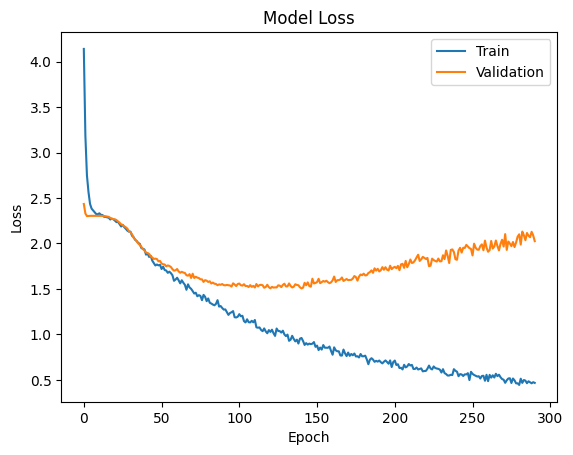
\includegraphics[width=5cm]{vl_loss.png}
\end{figure}

%Presentamos aqu\'i adem\'as la matriz de confusi\'on.

\begin{figure}[h!]
	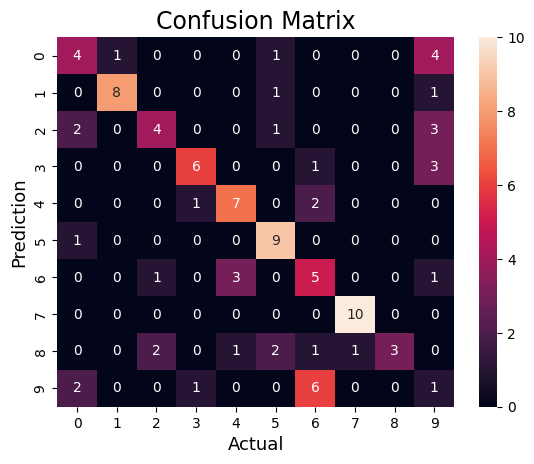
\includegraphics[width=5cm]{vl_confussion_matrix.png}
\end{figure}

Finalmente con un accuracy de $0.57$ y con valor para la funci\'on de p\'erdida de  $2.9323$ llegamos a la conclusi\'on de que este modelo no arroja resultados que mejoren los obtenidos en los modelos ya vistos antes.

	\section{Recomendaciones}
  
Un aspecto crítico que afecta el rendimiento de los modelos de clasificación radica en la precisión y consistencia de las anotaciones asignadas manualmente. Los esfuerzos futuros deberían priorizar la recopilación de datos de mayor calidad a través de pautas más estrictas, anotaciones de expertos o procedimientos de ratificación de colaboración colectiva.

Otro enfoque para impulsar el rendimiento de los modelos de clasificación de género es combinar múltiples modelos a través de ensembles. Al integrar predicciones de distintos algoritmos y representaciones de características, los ensembles aprovechan las fortalezas de los clasificadores individuales mientras mitigan sus debilidades.  

  Al seguir estas direcciones, los investigadores pueden ampliar nuestra comprensión de la clasificación de géneros musicales y sentar bases sólidas para soluciones de próxima generación en áreas relacionadas, incluido el análisis de audio, la recuperación de información o las interfaces interactivas centradas en el ser humano.
  
	    
	\begin{thebibliography}{20}
		\bibitem{whisper} A. Radford, J. Wook Kim, T. Xu, G. Brockman, C. McLeavey y I. Sutskever: \emph{RobustSpeechRecognitionviaLarge-ScaleWeakSupervision}. Preprint on arXiv: 2212.04356, 2022. 	
		\bibitem{Conv1D} Safaa Allamy, Alessandro Lameiras Koerich: \emph{1D CNN Architectures for Music Genre Classification}. Preprint on arXiv.2105.07302, 2021. 
		\bibitem{bert} J. Devlin, M. Chang, K. Lee y K. Toutanova: \emph{BERT:Pre-trainingofDeepBidirectionalTransformersfor LanguageUnderstanding}. Preprint on arXiv: 1810.04805, 2018. 
		\bibitem{murphy} Kevin P. Murphy: \emph{Machine Learning: A Probabilistic Perspective}. MIT Press, 2012.
		\bibitem{Wavelet Transform for Music Genre Classification} Pranav Vijaya Kumar Rao, Vishwas Nagesh Moolimani: \emph{ECG Analysis based feature extraction using Wavelet Transform for Music Genre Classification}, 2020. 
		\bibitem{wavelet transform in machine learning} Ahmet Taspinar: \emph{A guide for using the wavelet transform in machine learning}, unpublished. [Online]. Available: http://ataspinar.com/2018/12/21/a-guide-for-using-the-wavelet-transform-in-machine-learning/
		\bibitem{DT-CWT} Selesnick, I.W. and Baraniuk, R.G. and Kingsbury, N.C., \emph{The dual-tree complex wavelet transform}, 2005, IEEE Signal Processing Magazine, pp. 123-151.
		\bibitem{Wavelets y sus Aplicaciones} Liliana R. Castro, Silvia M.  Castro: \emph{Wavelets y sus Aplicaciones}, ler. Congreso Argentino de Ciencias de la Computación, pp. 195-204.
		\bibitem{Musical Genre Classification Of Audio Signals} George Tzanetakis, Georg Essl, Perry Cook: \emph{Automatic Musical Genre Classification Of Audio Signals}
		\bibitem{Machine Learning and Deep Learning methods for music genre Classification} Rusian Gohkman: \emph{Machine Learning and Deep Learning methods for music genre Classification}
    \end{thebibliography}
	
\end{document}
